\chapter{Development Process}
\label{chap:devprocess}

This chapter describes how the project was carried out in practice. It presents the chosen development methodology of the project, the weekly work rhythm that was followed, the role of feedback, the main project phases, and the tools that were used in the development.

%------------------------- 3.1 -------------------------

\section{Group Background and Project Organization}
\label{sec:group-background-and-project-organization}

This bachelor thesis is carried out by three students enrolled in the Bachelor’s program in Data Engineering at the Norwegian University of Science and Technology (NTNU). Throughout the study program, the group members have acquired foundational knowledge in programming, software engineering, databases, and system architecture. The project allows this knowledge to be applied in a practical context while also emphasizing structured collaboration, version control, and agile working methodologies.

The project reflects the group’s technical interests while also providing practical experience with \acrshort{ml} and computer vision. The group’s motivation stems from a shared interest in these fields, which were among the most engaging topics in the study program. This project made it possible to work with training and fine-tuning \acrshort{ml} models, while also developing computer vision solutions related to privacy and security in visual media. Through experimentation, evaluation, and iterative refinement, theoretical concepts were applied to real-world challenges related to privacy and automated redaction. In this way, the work contributed to both academic development and practical competence building.

Responsibility was divided among the group members to structure the workload, including Scrum coordination, product responsibility, documentation, and development. Henrik Weflen Gjermundsen had responsibility as Scrum Master and backend developer, Karwan Shekhe had responsibility as product manager and backend developer, and An Hoang Chu had responsibility as documentation manager and frontend developer. These roles gave the group an initial structure which helped communication, meeting notes and product direction. All members contributed as developers, and tasks were redistributed as the project required support across frontend, backend, testing, research and report writing. The projectplan Appendix~\ref{appsec:group} further describes the formal role distribution and group routines in detail.




The project involved both collaboration with Safe Media AI and supervision from NTNU. SafeVision was developed with representatives from Safe Media AI, Jon Yngve Hardeberg and Yasin Hessnawi. The project was supervised by Tom Røise, a university lecturer at the Department of Information Technology and Informatics at NTNU in Gjøvik, who provided guidance on methodological choices, technical challenges, and the overall direction of the project.


%------------------------- 3.2 -------------------------



%------------------------- 2.3 -------------------------

\section{Development Methodology}
\label{sec:project-team-and-methodology}

The development process was based on the Scrumban methodology, which is also described in the project plan in Appendix~\ref{appsec:pfar}. Scrumban combines Scrum-based sprint structure with Kanban-based workflow visualization and task-flow management \cite{bhavsar2020scrumban}. This approach suited the project because the work involved technical uncertainty and changing priorities throughout the development period. The team needed to adjust continuously as available technologies were explored and new input was received from the project owners. A fixed plan would have been too rigid for this kind of project, while an unstructured process would have made coordination and progress tracking difficult.

Scrum was used to create a structured and adaptable development process. The work was organized into mostly one-week sprints, with some longer sprints later once the direction of the final project became clearer. This gave the group manageable planning periods in the early phases and made it possible to adapt when the work shifted from research and prototyping to integration and refinement. As outlined in the project plan in Appendix~\ref{appsec:pfar}, the sprint structure was supported by regular meetings, task distribution, and weekly logging, which made progress easier to track and helped keep the project aligned between the group members, the supervisor, and Safe Media AI.

\begin{figure}[H]
\centering
\resizebox{\textwidth}{!}{%
\begin{tikzpicture}[
    proc/.style={
        draw,
        rounded corners=2pt,
        fill=blue!10,
        align=center,
        minimum width=2.9cm,
        minimum height=1cm,
        font=\small
    },
    column/.style={
        draw,
        rounded corners=2pt,
        fill=gray!10,
        align=center,
        minimum width=2.1cm,
        minimum height=1cm,
        font=\small
    },
    ext/.style={
        draw,
        rounded corners=2pt,
        fill=green!10,
        align=center,
        minimum width=3.0cm,
        minimum height=0.9cm,
        font=\small
    },
    arrow/.style={-{Latex[length=2.2mm]}, thick},
    feedback/.style={-{Latex[length=2.2mm]}, thick, dashed}
]

% Feedback sources
\node[ext] (internal) at (1.4,4.2) {Internal team\\coordination};
\node[ext] (supervisor) at (5.0,4.2) {Supervisor\\feedback};
\node[ext] (commissioner) at (8.6,4.2) {Safe Media AI AS\\feedback};

% Sprint planning and backlog
\node[proc] (planning) at (1.4,2.1) {Sprint\\planning};
\node[proc] (backlog) at (5.0,2.1) {Sprint backlog\\and task selection};

% Kanban board background (moved slightly lower)
\draw[
    rounded corners=3pt,
    draw,
    fill=blue!4
] (6.8,-0.2) rectangle (19.1,2.4);

\node[font=\small\bfseries] at (12.95,1.95) {Jira / Kanban workflow};

% Kanban columns (moved lower)
\node[column] (todo) at (8.0,0.75) {To do};
\node[column] (progress) at (10.4,0.75) {In progress};
\node[column] (test) at (12.8,0.75) {To test};
\node[column] (review) at (15.2,0.75) {Review};
\node[column] (done) at (17.6,0.75) {Done};

% Main flow
\draw[arrow] (planning) -- (backlog);
\draw[arrow] (backlog) -- (todo);
\draw[arrow] (todo) -- (progress);
\draw[arrow] (progress) -- (test);
\draw[arrow] (test) -- (review);
\draw[arrow] (review) -- (done);

% Feedback arrows
\draw[feedback] (internal.south) -- (planning.north);
\draw[feedback] (supervisor.south) -- (backlog.north);
\draw[feedback] (commissioner.south) -- (backlog.north east);

\end{tikzpicture}%
}
\caption{Scrumban workflow used in the project, combining sprint-based planning with a Kanban task flow and feedback-based reprioritization.}
\label{fig:scrumban-workflow}
\end{figure}

Kanban contributed to flexible development by giving the team continuous visibility of the workflow. Tasks were created as issues through the Jira board and followed a flow where they moved from planning to active work, testing, review and completion. In this way, it became easier to reprioritize when new tasks appeared, when the group received feedback from the supervisor or Safe Media AI, or when obstacles came up during development. Kanban therefore supported a more adaptive process than a sprint plan alone could have provided.

\begin{figure}[H]
    \centering
    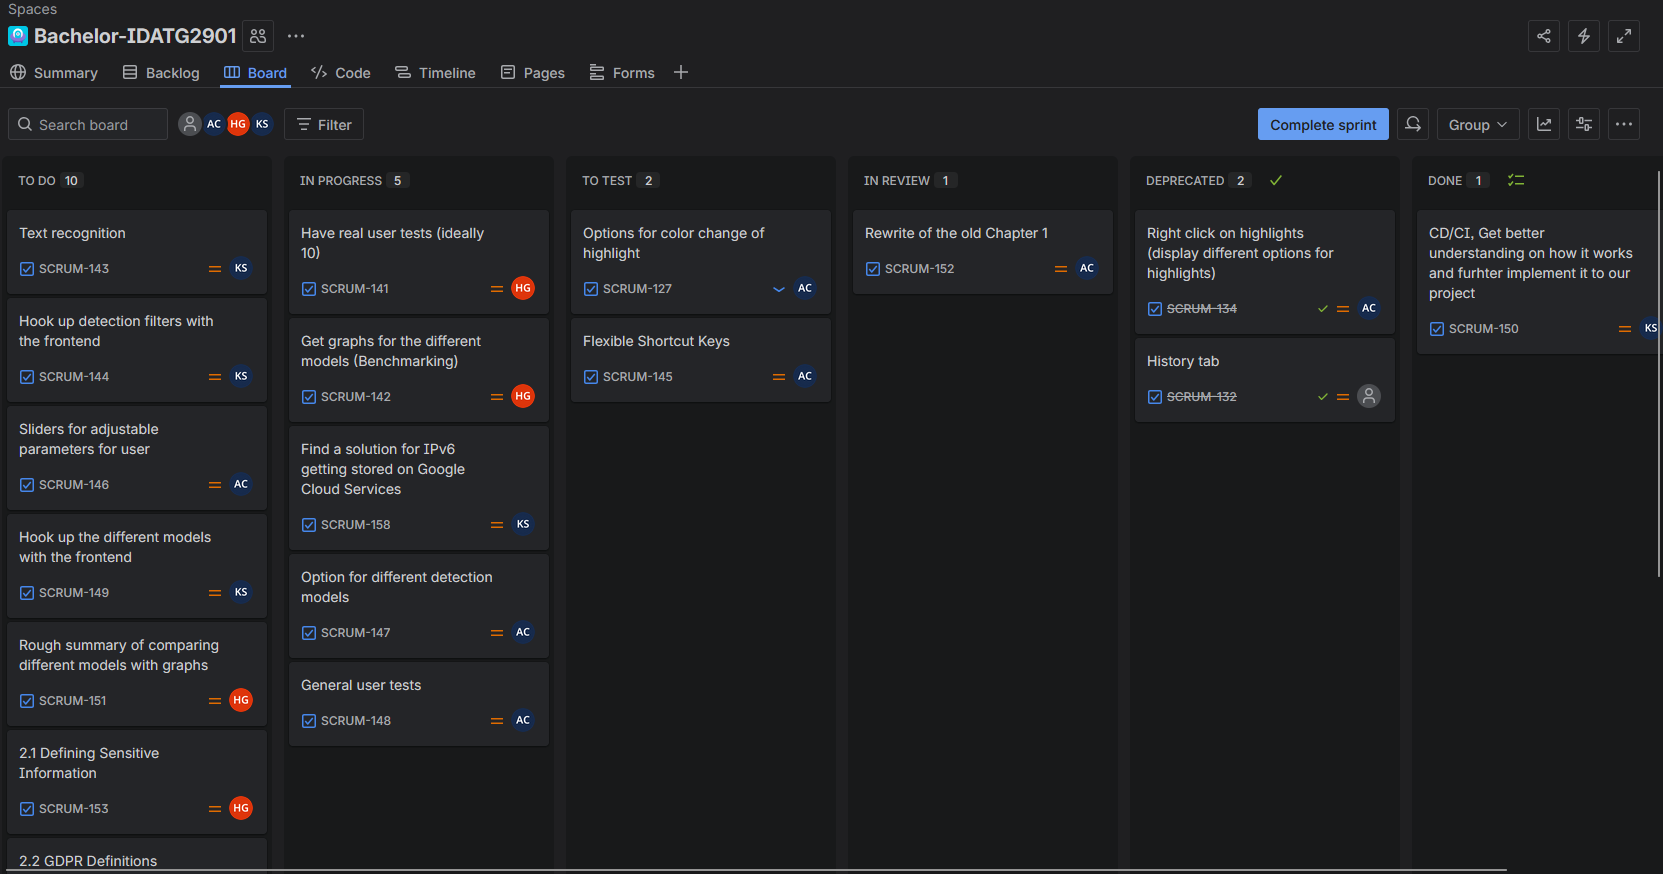
\includegraphics[width=\linewidth]{figures/images/chapter-4/jira_week9.jpg}
    \caption{Jira board snapshot from Week 9, showing active work related to feature development, testing and refinement.}
    \label{fig:jira-week9}
\end{figure}

In practice, the methodology was implemented through short sprint cycles, frequent internal coordination and regular reviews. Together, Scrum and Kanban provided a structured and adaptable development process (Figure~\ref{fig:scrumban-workflow}). This was important in a project where technical choices, feature priorities and implementation details had to be adjusted throughout. The use of Scrumban made it possible to maintain progress and direction, while still leaving room for change.


\section{Sprint Structure and Weekly Project Rhythm}

This section describes the weekly work rhythm and how it functioned in practice. It explains how the group worked in a structured and consistent way with sprint planning, daily coordination and regular review points. This rhythm followed the routines described in the project plan, where sprint planning, daily Scrum, sprint reviews and retrospectives were defined as part of the working method, see Appendix~\ref{app:project-plan}.

\methodheading{Sprint Planning and Task Management}

Each sprint began with sprint planning, where the group decided which tasks should be prioritized in the coming work. In the early stages of the project, this process was mainly used to discuss project planning, assignment clarification, administrative setup, and the distribution of research tasks. Later, when the direction of the project had become clearer, sprint planning was used to divide work related to implementation, integration, testing, refinement, and report writing. This gave the team a clear short-term direction and made the project easier to manage step by step. Tasks were assessed through group discussion based on expected complexity, uncertainty, and available capacity. Larger tasks were divided into smaller issues when they became too broad to assign or complete within a sprint.

Tasks created in sprint planning were tracked as issues on the project’s issue board, where they were assigned to group members corresponding to the planning, Figure~\ref{fig:jira-week9}. This made it easier to divide larger goals discussed into smaller work tasks which could coexist with other new findings or technical challenges. Sprint planning therefore functioned both as coordination and as a way of keeping the tasks manageable. The planned sprint rhythm and meeting structure were defined in the project plan, including sprint planning, daily Scrum, sprint reviews and retrospectives, see Appendix~\ref{app:project-plan}.

\methodheading{Daily Coordination and Follow-Up}

Daily Scrum was used to maintain alignment within the group between sprint planning and weekly review meetings. The group contract in Appendix~\ref{app:project-plan} describes the routines established for frequent internal follow-up meetings throughout the week. These meetings were used to clarify completed work, ongoing tasks, and any blockers that needed to be addressed before the next milestone.

This continuous coordination was especially useful in a project where technical choices, implementation details and scope questions developed over time. In addition to daily Scrum, the group also worked together physically and digitally to solve problems and prepare for meetings. The daily coordination therefore helped maintain momentum in the project and the development process coherent.

\methodheading{Sprint Reviews and Retrospectives}

Sprint reviews and retrospectives were closely tied to the meeting with the supervisor and Safe Media AI. These meetings worked as natural review points for the group where status was presented, feedback was received, and afterwards a discussion of how the project can move forward. Input from these weekly sessions was often used directly to adjust scope, clarify technical direction and decide what should be prioritized in the coming sprint.

This structure gave the team a continuous opportunity to reflect on the product and the process. What had worked well, what had created problems and what was the strategy going to be in the coming phase. In this way, the review structure also supported continuous improvement throughout the project. The sprint reviews did not only mark the end of one work period, but they became an important mechanism for learning and helped connect weekly development to broader academic and practical expectations.

%------------------------- 3.4 -------------------------

\section{Stakeholder Involvement}
\label{sec:stakeholder-involvement-external-feedback}

Throughout the project, feedback from both the supervisor and Safe Media AI helped shape the direction, scope, and priorities of the work. Selected meetings that influenced the development process are summarized in Table~\ref{tab:meeting-impact}, while the full selected meeting notes are included in Appendix~\ref{app:meeting-notes}. The feedback was important not only for deciding which features to develop, but also for determining which ideas should remain outside the final scope. This helped the group prioritize relevant tasks, avoid unnecessary expansion of the system, and connect the technical development to both practical needs and academic expectations.

\begingroup
\scriptsize
\setlength{\tabcolsep}{3pt}
\renewcommand{\arraystretch}{1.08}
\setlength{\LTpre}{0.4em}
\setlength{\LTpost}{0.4em}

\begin{xltabular}{\textwidth}{
    >{\raggedright\arraybackslash}p{2.7cm}
    >{\raggedright\arraybackslash}X
}
\caption{Condensed overview of selected project meetings and their influence on project decisions.}
\label{tab:meeting-impact}\\

\toprule
\textbf{Date and type} & \textbf{Main outcome and project impact} \\
\midrule
\endfirsthead

\toprule
\textbf{Date and type} & \textbf{Main outcome and project impact} \\
\midrule
\endhead

\midrule
\multicolumn{2}{r}{\footnotesize Continued on next page} \\
\endfoot

\bottomrule
\endlastfoot

\meetingcell{08.01.2026}{Internal group meeting}{app:meeting-2026-01-08}
& Established the initial project structure, including administrative setup, role distribution, Scrum routines, work logging, GitLab issues, Overleaf documentation and the need for a group contract. \\

\meetingcell{09.01.2026}{Internal group meeting}{app:meeting-2026-01-09}
& The group decided to pursue the Safe Media AI AS assignment as the preferred project direction, contacted the commissioner and prioritized completing enough of the project plan to receive early supervisor feedback. \\

\meetingcell{15.01.2026}{Startup meeting with commissioner}{app:meeting-2026-01-15}
& Clarified the assignment direction with Safe Media AI AS. Image redaction became the main starting point, React or Vue was recommended for the frontend, Python for the backend, and faces and text were identified as early detection priorities. \\

\meetingcell{22.01.2026}{Commissioner meeting}{app:meeting-2026-01-22}
& Defined the integration boundary more clearly. The group should limit the core system to image-based redaction, while Safe Media AI AS' existing system could handle document-level PDF workflows. Manual user correction was emphasized as a core requirement. \\

\meetingcell{26.01.2026}{Supervisor meeting}{app:meeting-2026-01-26}
& Received feedback on the project plan and report direction. The supervisor emphasized academic justification of technical choices and recommended using an early throwaway prototype to explore tools before committing to the real MVP. \\

\meetingcell{29.01.2026}{Commissioner meeting}{app:meeting-2026-01-29}
& Presented early prototype progress and agreed on closer weekly commissioner involvement. The meeting influenced later work on redaction strength, privacy, user trust, possible video tracking and research into \acrshort{gdpr} and \gls{anonymization} practice. \\

\meetingcell{09.02.2026}{Supervisor meeting}{app:meeting-2026-02-09}
& Clarified the evaluation priorities. The supervisor emphasized testing both correct and incorrect detections, documenting model quality with evidence, checking model licensing and considering privacy risks related to image and video processing. \\

\meetingcell{12.02.2026}{Commissioner meeting}{app:meeting-2026-02-12}
& Confirmed that full PDF handling should remain outside the core backend because Safe Media AI AS already handled PDF extraction. The meeting reinforced image-based processing, \acrshort{ocr}/text detection, performance expectations, private repositories and early deployment planning. \\

\meetingcell{16.02.2026}{Supervisor meeting}{app:meeting-2026-02-16}
& Supported moving PDF handling into project limitations and defining image redaction as the main subject of the report. The supervisor encouraged deeper technical evaluation of speed, privacy, model quality, parallel detection and relevant scientific literature. \\

\meetingcell{19.02.2026}{Commissioner meeting}{app:meeting-2026-02-19}
& Influenced feature priorities for the MVP, including file-format support, improved text detection, filter options, manual marking, adjustable highlight boxes, response structure, benchmarking, user testing and possible ground-truth data collection. \\

\meetingcell{05.03.2026}{Commissioner meeting}{app:meeting-2026-03-05}
& Explored video, advanced options and practical user needs. Video was considered relevant but secondary, while expert-mode options, interface complexity and real-world redaction workflows were identified as important design considerations. \\

\meetingcell{09.03.2026}{Supervisor meeting}{app:meeting-2026-03-09}
& Refined the user-test plan. The supervisor advised that the test should support evaluation rather than sales, assess the basic image workflow, use clear tasks and images, and treat video mainly as a proof of concept or future direction. \\

\meetingcell{18.03.2026}{Commissioner meeting}{app:meeting-2026-03-18}
& Clarified Application Programming Interface (\acrshort{api}) based integration with Safe Media AI AS and the need to consider memory use, processing time and computational requirements. The meeting also narrowed video-related goals and emphasized feasible scope control. \\

\meetingcell{23.03.2026}{Supervisor meeting}{app:meeting-2026-03-23}
& Helped control the project scope after many explored directions, including JPEG, PNG, PDF, video, metadata and surveys. The supervisor advised defining detection and redaction as the main content of the report, with less central experiments moved to appendices. \\

\meetingcell{13.04.2026}{Supervisor meeting}{app:meeting-2026-04-13}
& Provided report feedback for the remaining project period. The supervisor emphasized improving the abstract and summary, connecting theory more directly to the project, strengthening GDPR and sensitive-information discussion, and explaining development-process choices rather than only listing chronology. \\

\meetingcell{22.04.2026}{Guidance for user testing and UI design}{app:meeting-2026-04-22}
& Provided feedback on user communication during processing, video settings, report framing, benchmarking and interface terminology. The meeting also clarified that \gls{inpainting} should be presented as part of the explored and implemented functionality if the achieved results were usable. \\

\meetingcell{23.04.2026}{Supervisor meeting}{app:meeting-2026-04-23}
& Set the final phase priorities as report quality, testing, figures and security. The supervisor recommended improving readability, clearly discussing figures, showing implementation progress, documenting implemented security measures and avoiding unnecessary new functionality near the deadline. \\

\end{xltabular}

\vspace{0.3em}
\noindent\footnotesize\textit{Note.} This table presents a summary of selected meeting notes. The meeting content was summarized with artificial intelligence and reviewed by the project group.

\endgroup

The supervisor contributed mainly through guidance on group structure, prioritization, documentation, and report writing. This became especially important after the group had developed a working version of the system and began considering possible extensions. Through these discussions, the group was encouraged to document added functionality properly rather than trying to include every explored idea in the final product. Several meetings were also used to review report chapters and clarify what belonged in the main thesis.

Safe Media AI contributed mainly to the practical and product-oriented direction of the project. Their feedback helped clarify the project scope, feature priorities, integration boundaries, and expectations for the delivered prototype. This ensured that the development process was connected to practical needs rather than only the group’s own assumptions. 


\section{Project Timeline and Milestone Development}
\label{sec:project-timeline-milestones}

Figure~\ref{fig:project-timeline} summarizes the main phases of the project from January to May. The timeline is divided into five phases, showing how the work developed from assignment clarification and early exploration to implementation, user feedback, scope narrowing, and final documentation.

\begin{figure}[H]
\centering
\resizebox{\textwidth}{!}{%
\begin{tikzpicture}[
    phase/.style={
        draw,
        rounded corners=2pt,
        align=left,
        minimum height=0.9cm,
        font=\small
    }
]

% Main timeline
\draw[thick] (0,0) -- (15,0);

% Month ticks and labels
\foreach \x/\m in {0/Jan.,3/Feb.,6/Mar.,9/Apr.,12/May}
{
    \draw[thick] (\x,0.18) -- (\x,-0.18);
    \node[font=\small\bfseries] at (\x,-0.55) {\m};
}
\draw[thick] (15,0.18) -- (15,-0.18);

% Phase boxes below the timeline
\node[phase, fill=blue!15, anchor=west, minimum width=3.2cm] at (0.2,-1.4)
{\textbf{A.} Kickoff, assignment change\\and scope clarification};

\node[phase, fill=green!15, anchor=west, minimum width=4.8cm] at (1.0,-2.5)
{\textbf{B.} Research, literature review,\\prototyping and MVP exploration};

\node[phase, fill=orange!15, anchor=west, minimum width=5.2cm] at (4.0,-3.6)
{\textbf{C.} Feature implementation, \acrshort{ocr},\\manual editing, filters and testing};

\node[phase, fill=purple!15, anchor=west, minimum width=4.5cm] at (6.6,-4.7)
{\textbf{D.} External feedback, user testing\\and practical refinement};

\node[phase, fill=red!15, anchor=west, minimum width=5.2cm] at (8.4,-5.8)
{\textbf{E.} Scope narrowing, final refinement,\\report writing and documentation};

\end{tikzpicture}%
}
\caption{Project timeline showing the main phases from assignment clarification to final refinement and documentation.}
\label{fig:project-timeline}
\end{figure}

The first phase consisted of kickoff, assignment change, and scope clarification. The project began with a transition period involving a change in assignment, role organization, and initial planning with the supervisor. During the first weeks, the group briefly collaborated with a different external client, but the cooperation was discontinued at an early stage. After securing the new assignment with Safe Media AI, the group prioritized scope clarification and early research. The team discussed what the solution should address, how sensitive information should be understood in visual media, and which technical and practical boundaries needed to be defined from the start. This transition is documented in the project plan in Appendix~\ref{app:project-plan}.

The second phase focused on research, literature review, prototyping, and MVP exploration. During this stage, the group investigated relevant models, datasets, and technical approaches that could support the final solution. Early frontend and backend prototypes were tested to explore possible implementation directions. The goal of this phase was to identify a workable technical foundation and establish an MVP that could guide further development.

The third phase centered on feature implementation and technical expansion. After the MVP had established a more stable foundation, the work shifted from exploration to building functionality on top of the existing system. This included image-based detection and redaction, \acrshort{ocr} and text processing, manual editing of \gls{bounding box}es, filtering options, redaction modes, deployment work, and testing. During this phase, the system evolved from an early prototype into a more complete and usable application.

The fourth phase emphasized external feedback and user testing. A meeting with Skan-Kontroll gave the group insight into how redaction could be relevant in practical workflows, while UX guidance from Thomas Berg Fjellestad contributed feedback on interface clarity and workflow design. Together with the group’s own testing, this phase helped evaluate usability and practical relevance. The structured user testing itself is discussed separately in Section~\ref{sec:user-testing}.

The final phase consisted of scope narrowing, final refinement, report writing, and documentation. Several possible directions had been explored during development, including video support, benchmarking, QR and barcode detection, metadata-related handling, and interface refinement. At this stage, the group prioritized the most achievable and relevant deliverables, with the image based workflow remaining the core functionality of the system.

\section{Tools and Working Practices}
\label{sec:tools-and-working-practices}

The project was supported by a set of tools for communication, planning, documentation, and practical collaboration. These tools helped structure the development process and supported both the technical work and the written thesis. Rather than being part of the system itself, they were used to coordinate tasks, document progress, and support the group’s daily workflow.

\begin{table}[H]
\centering
\caption{Main tools used to support project work}
\label{tab:project_tools}
\begin{tabular}{p{3.2cm} p{10.2cm}}
\toprule
\textbf{Tool} & \textbf{Purpose in the project} \\
\midrule
Jira & Planning, task distribution, and issue tracking \\

GitHub & Version control and collaborative code management \\

Figma & Creation of low-fidelity wireframes for early interface design \\

Excel & Hour logging and short weekly summaries of completed work \\

Discord & Internal communication within the group \\

draw.io & Creation of diagrams and figures \\

LaTeX / Overleaf & Thesis writing and report formatting \\

Word & Supporting documentation and meeting material \\

VS Code & Shared development environment for implementation work \\
\bottomrule
\end{tabular}
\end{table}

Jira was used for planning and issue tracking, which supported the Scrumban-based work process. GitHub was used for version control and collaborative code management, while VS Code was the shared development environment used by the group. Discord and physical meetings were used for internal communication, and Teams was used in several meetings with Safe Media AI AS.

\begin{figure}[H]
    \centering
    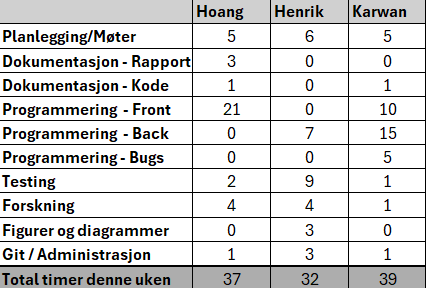
\includegraphics[width=0.95\textwidth]{figures/images/chapter-3/timeliste.png}
    \caption{Example from the project hour list, showing work distribution during week 9.}
    \label{fig:project_hour_list_example}
\end{figure}

Documentation and reporting were supported through LaTeX in Overleaf, together with Word and Excel (Figure~\ref{fig:project_hour_list_example}) for supplementary project material such as meeting notes and hour logging, further detailed spreadsheet for the hour list is in Appendix~\ref{app:project-hour-tracking}. In addition, Figma was used to sketch low-fidelity wireframes, and draw.io was used to create diagrams and figures. A summary of the main tools used in the project is provided in Table~\ref{tab:project_tools}.

\begin{figure}[H]
    \centering
    \makebox[\textwidth][c]{%
        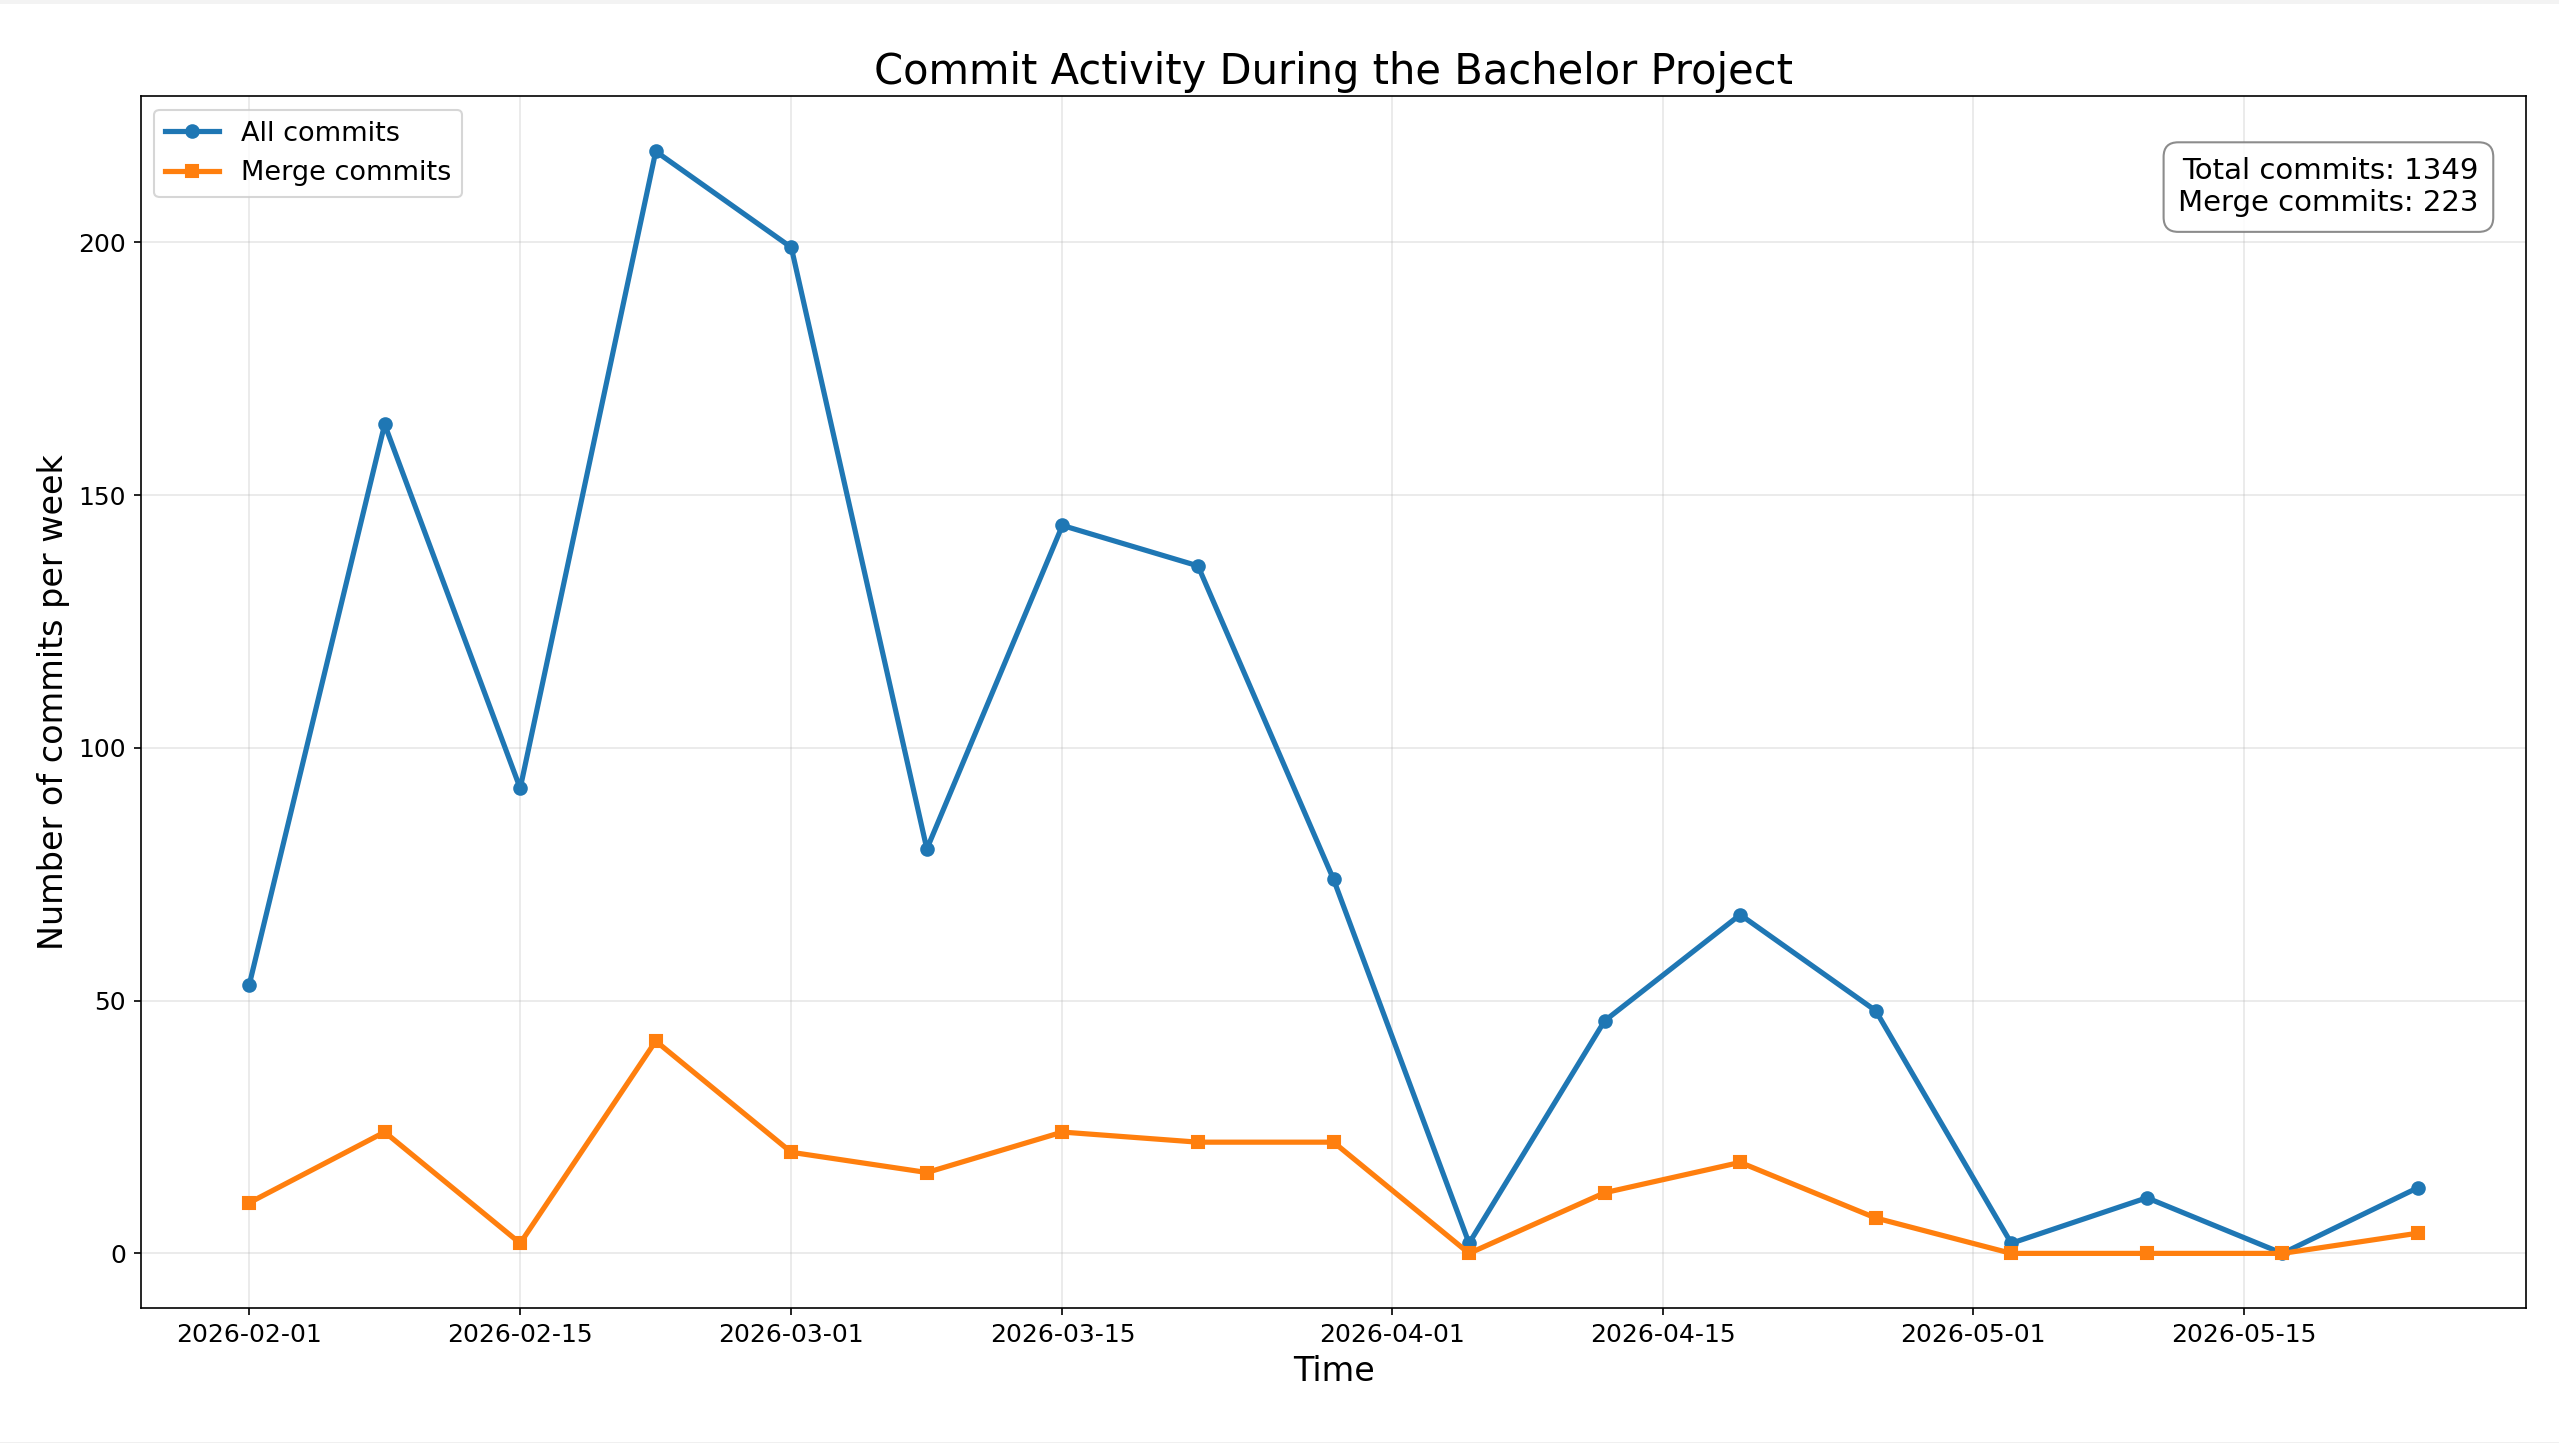
\includegraphics[width=1.3\linewidth]{figures/images/chapter-3/commit_merge_timeline.png}%
    }
    \caption{GitHub commit activity during the project period, showing how implementation work was distributed over time.}
    \label{fig:github_commit_timeline}
\end{figure}

The GitHub commit history provides an overview of the actual implementation activity during the project. Figure~\ref{fig:github_commit_timeline} shows how development work was distributed over time, including periods of higher implementation intensity and later refinement. The timeline supports the project history described in this chapter by showing that development was carried out continuously rather than being concentrated only near the end of the project.

\section{Artificial Intelligence as a Development Tool}
\label{sec:ai-development-tool}

Artificial intelligence was used as a supporting tool throughout the project, but not as an independent decision maker. Its role was to provide suggestions, help clarify problems, and reduce time spent on repetitive or clearly defined tasks. All outputs that affected the system, report, or technical decisions were reviewed, tested, and adapted by the group before being included.

In development work, the support mainly involved code review, error explanation, alternative implementation suggestions, and smaller debugging tasks. Generated code was not copied directly into the system without evaluation since the suggestions often had to be adjusted to fit the existing architecture and implementation choices. The tools also contributed to code documentation by helping formulate explanations of selected implementation details.

For technical research and problem solving, AI helped compare possible approaches and identify relevant technologies or methods. This was useful when the group needed an initial overview of different implementation alternatives before evaluating them more critically. In the \acrshort{ml} part of the project, synthetic text examples were generated for the text classification pipeline, including examples of sensitive and non-sensitive text entities. These examples were treated as supporting material and reviewed before use.

In the report work, AI contributed to spelling correction, sentence reformulation, clarification of technical explanations, and troubleshooting of LaTeX or Overleaf compiler errors. The final wording, technical content, and project decisions remained the responsibility of the group, and the suggestions were adjusted to match the actual implementation and writing style of the thesis.
